\chapter{เอกสารสำคัญที่เกี่ยวข้อง}
\begin{itemize}
    \item \textbf{เอกสารสำคัญของคณะ}
          \begin{itemize}
              \item \hyperlink{target:approval}{หนังสือยินยอมให้เผยแพร่รายงานปฏิบัติงานสหกิจศึกษา} (หน้า \pageref{page:approval})
              \item \hyperlink{target:03-04}{วศ.สก.-03/04 รายงานตัวเข้าสหกิจศึกษา} (หน้า \pageref{page:03-04})
              \item \hyperlink{target:06}{วศ.สก-06 แบบแจ้งโครงร่างรายงานการปฏิบัติงานสหกิจศึกษา} (หน้า \pageref{page:06})
              \item \hyperlink{target:10}{วศ.สก-10 แบบสรุปการปฏิบัติงานสหกิจศึกษาประจาสัปดาห์} (หน้า \pageref{page:10})
              \item \hyperlink{target:11}{วศ.สก.-11 แบบสรุปผลการปฏิบัติงานสหกิจศึกษา} (หน้า \pageref{page:11})
          \end{itemize}
    
    \item \textbf{เอกสารสำคัญที่เกี่ยวข้องกับงาน}
          \begin{itemize}
              \item \hyperlink{target:create}{เอกสารสรุปโปรแกรมที่สร้าง} (หน้า \pageref{page:create})
              \item \hyperlink{target:angular}{เอกสารสรุปสิ่งที่ได้เรียนรู้และลองทำ Angular} (หน้า \pageref{page:angular})
              \item \hyperlink{target:springboot}{เอกสารสรุปสิ่งที่ได้เรียนรู้และลองทำ Java Spring Boot} (หน้า \pageref{page:springboot})
              \item \hyperlink{target:sqlserver}{เอกสารสรุปสิ่งที่ได้เรียนรู้และลองทำ SQL Server} (หน้า \pageref{page:sqlserver})

          \end{itemize}

\end{itemize}

% คณะ

\includepdf[pages=-, scale=.8, pagecommand={\hypertarget{target:approval}{},\label{page:approval}}, nup=1x1, frame=false]{pdf/approval}

\includepdf[pages=-, scale=.8, pagecommand={\hypertarget{target:03-04}{},\label{page:03-04}}, nup=1x1, frame=false]{pdf/03-04_flat}

\includepdf[pages=-, scale=.8, pagecommand={\hypertarget{target:06}{},\label{page:06}}, nup=1x1, frame=false]{pdf/06_flat}
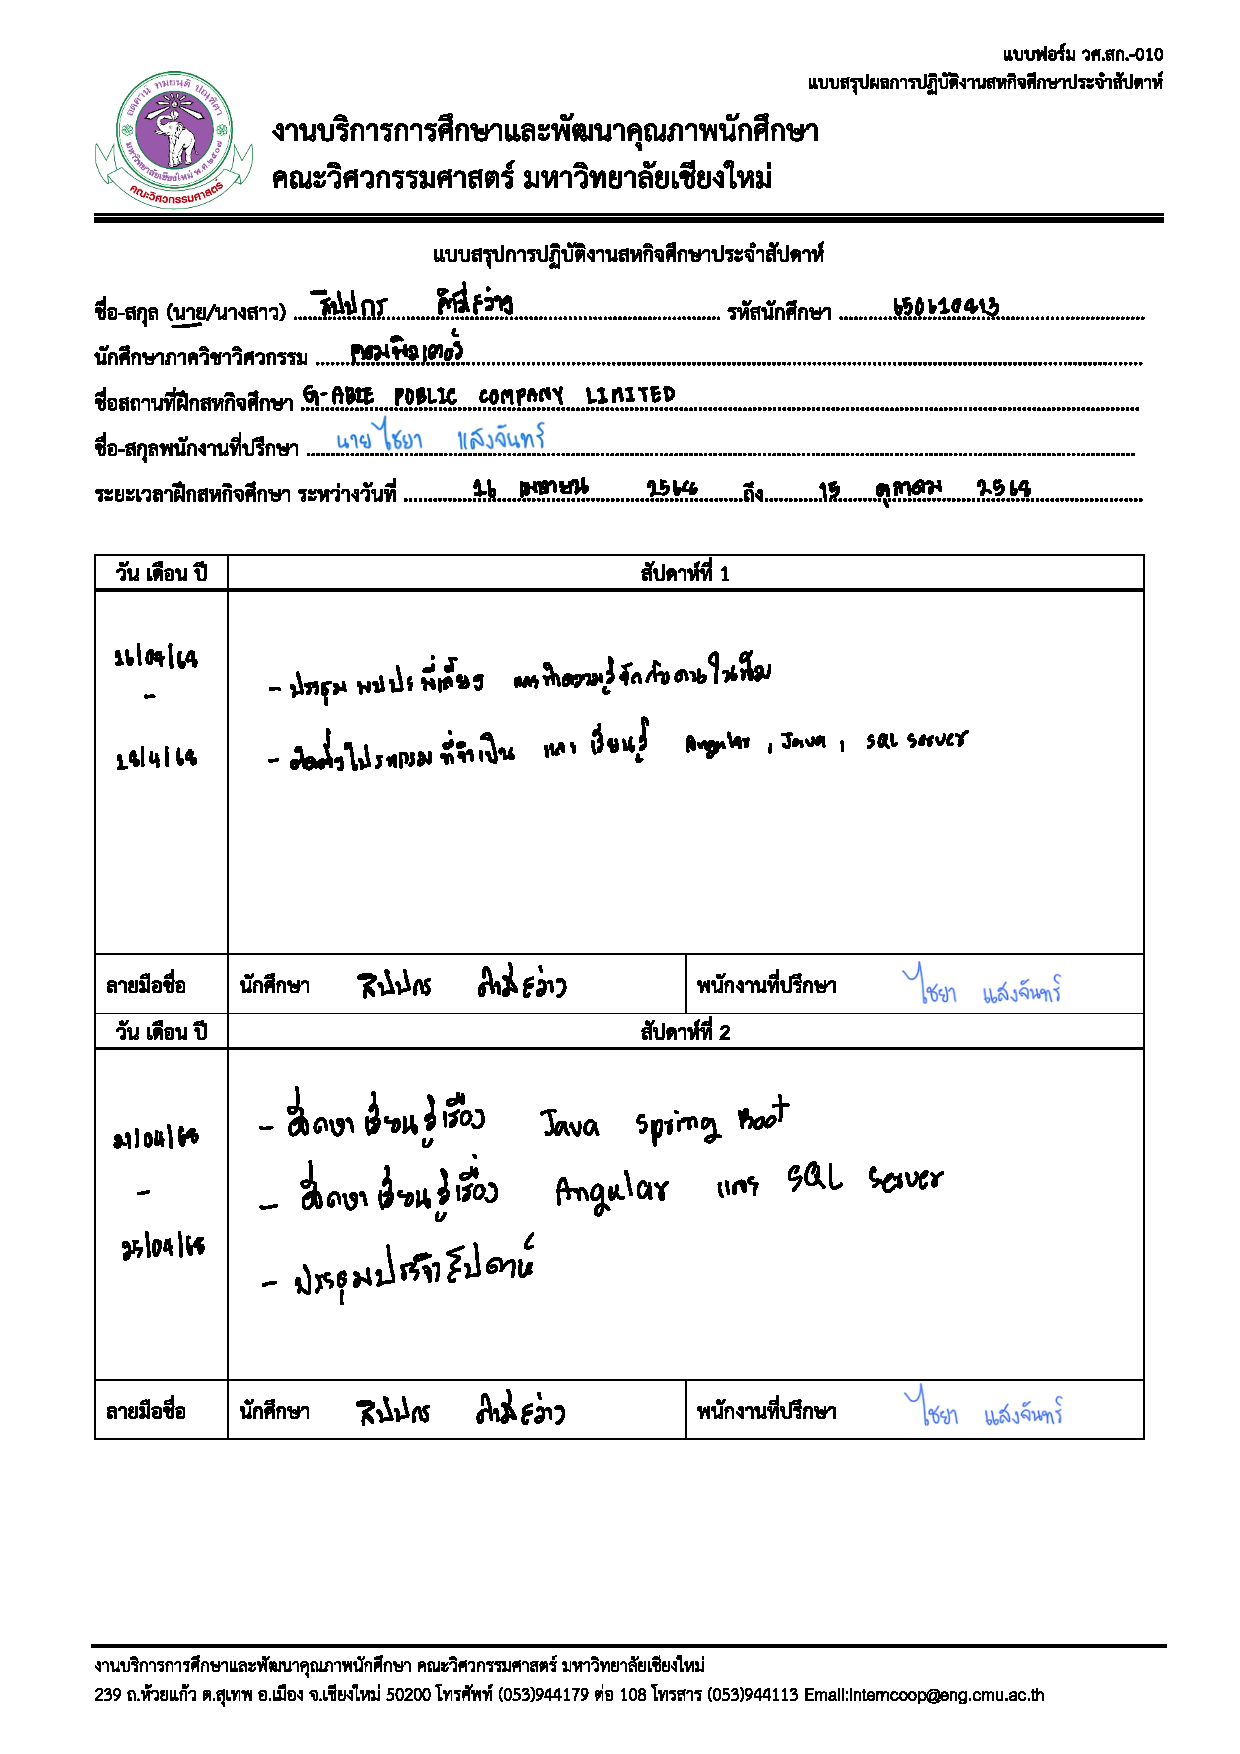
\includepdf[pages=-, scale=.8, pagecommand={\hypertarget{target:10}{},\label{page:10}}, nup=1x1, frame=false]{pdf/10_flat}

\includepdf[pages=-, scale=.8, pagecommand={\hypertarget{target:11}{},\label{page:11}}, nup=1x1, frame=false]{pdf/11_flat}

% ส่วนที่เกี่ยวข้อง
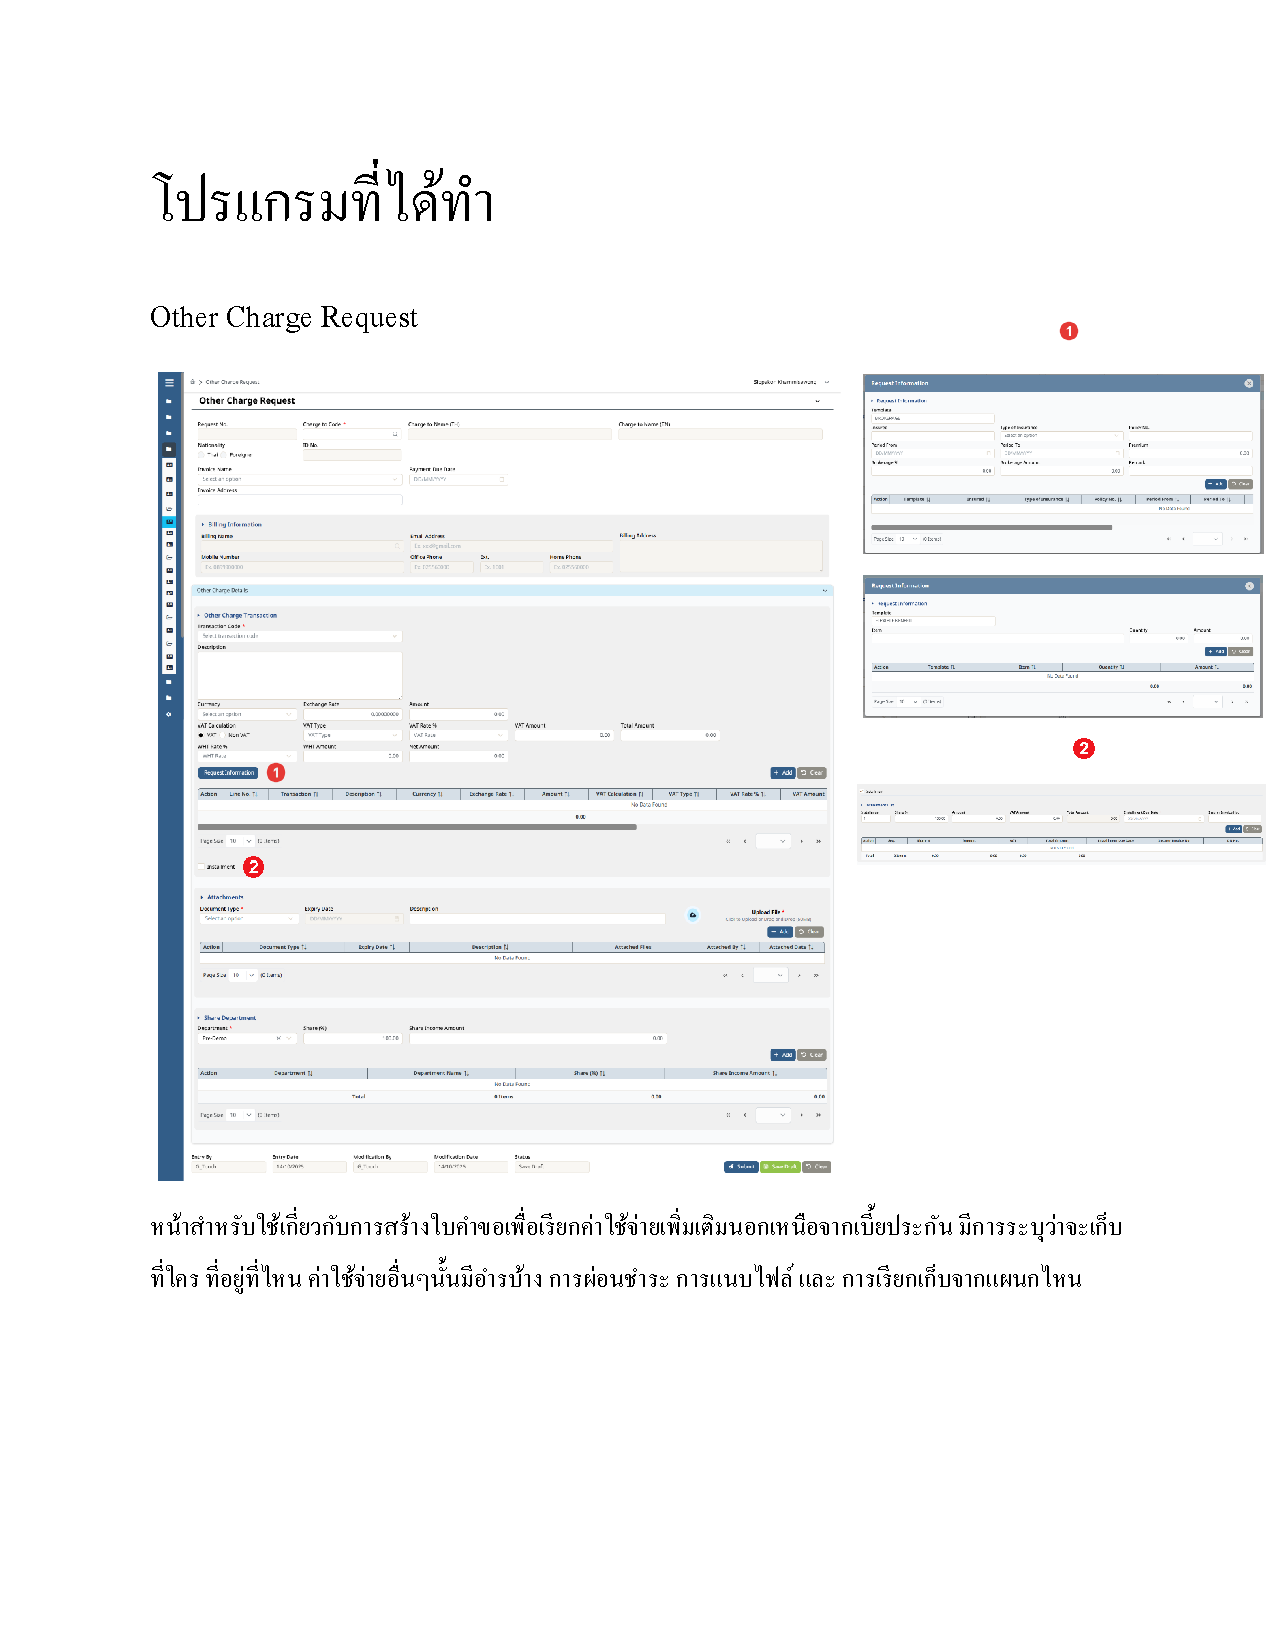
\includepdf[pages=-, scale=.8, pagecommand={\hypertarget{target:create}{},\label{page:create}}, nup=1x1, frame=false]{pdf/create}

\includepdf[pages=-, scale=.8, pagecommand={\hypertarget{target:angular}{},\label{page:angular}}, nup=1x1, frame=false]{pdf/angular}
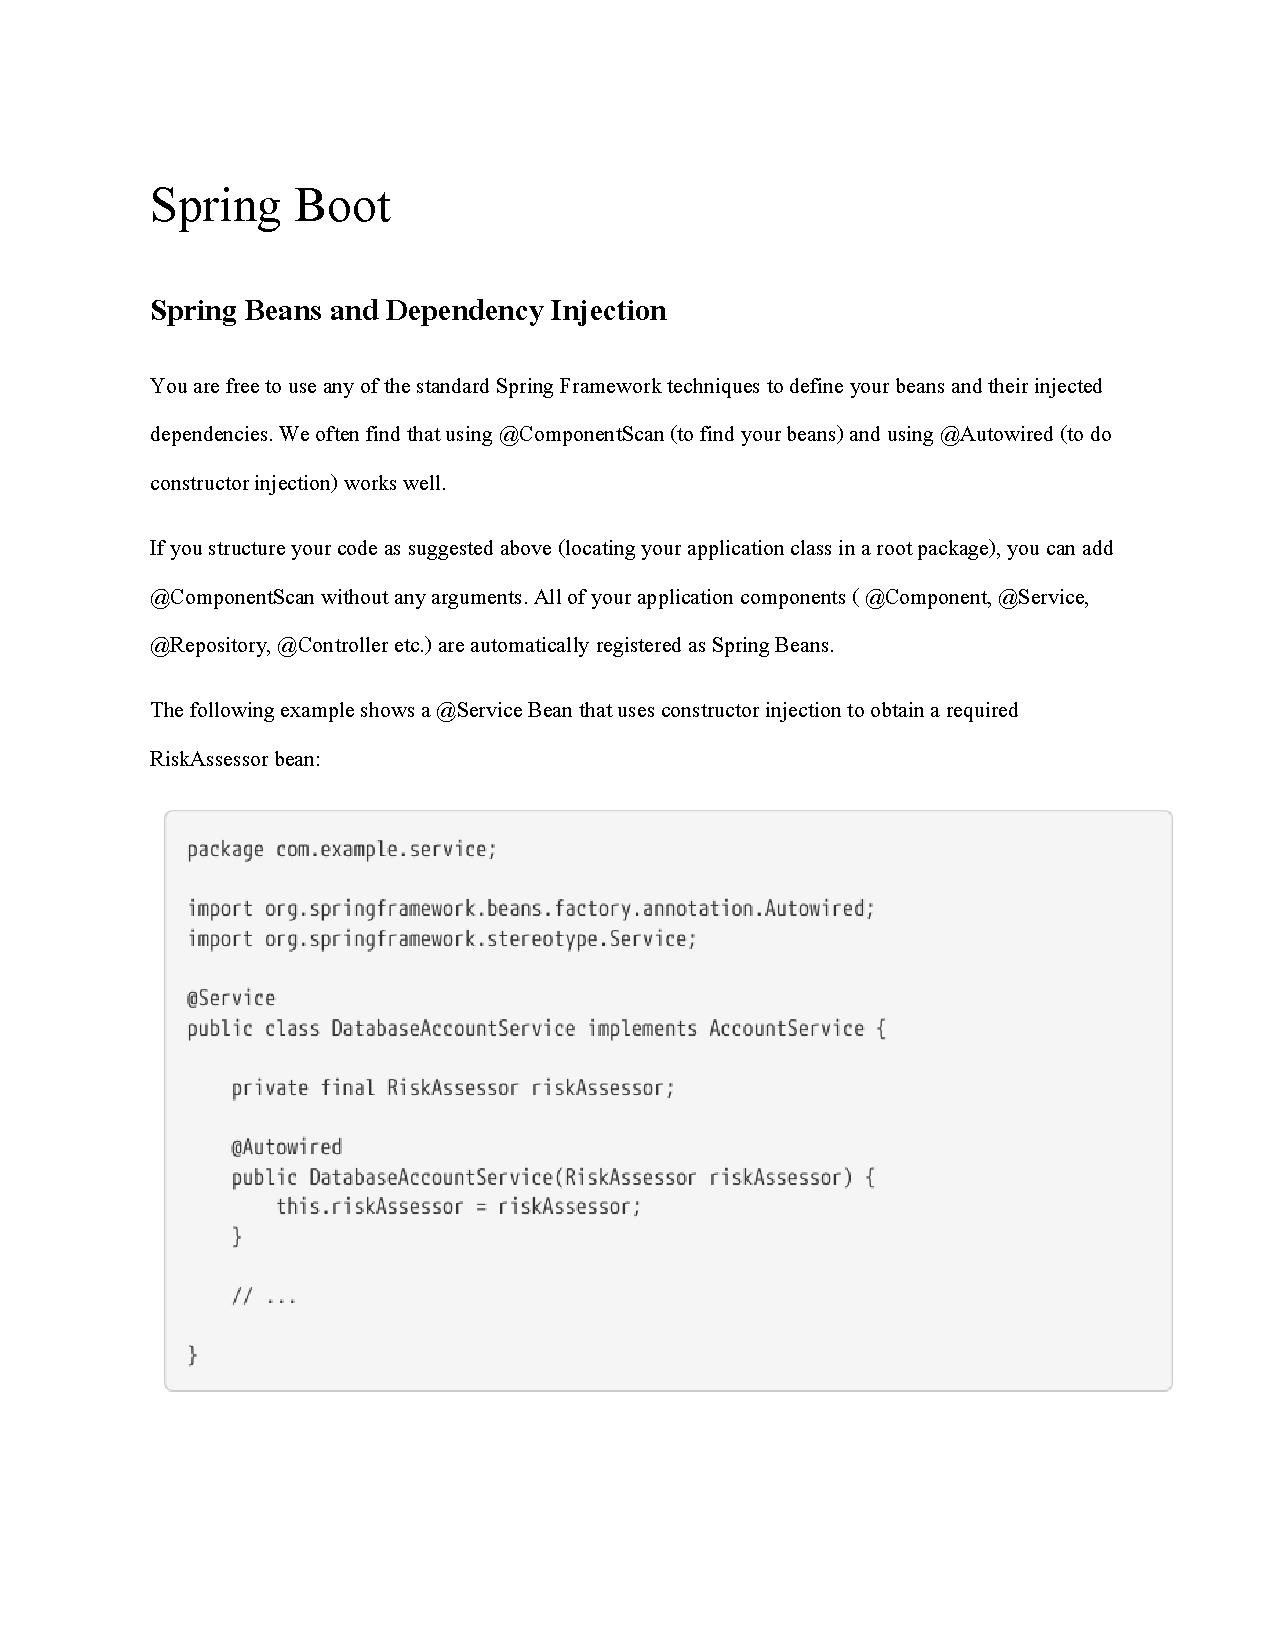
\includepdf[pages=-, scale=.8, pagecommand={\hypertarget{target:springboot}{},\label{page:springboot}}, nup=1x1, frame=false]{pdf/springboot}
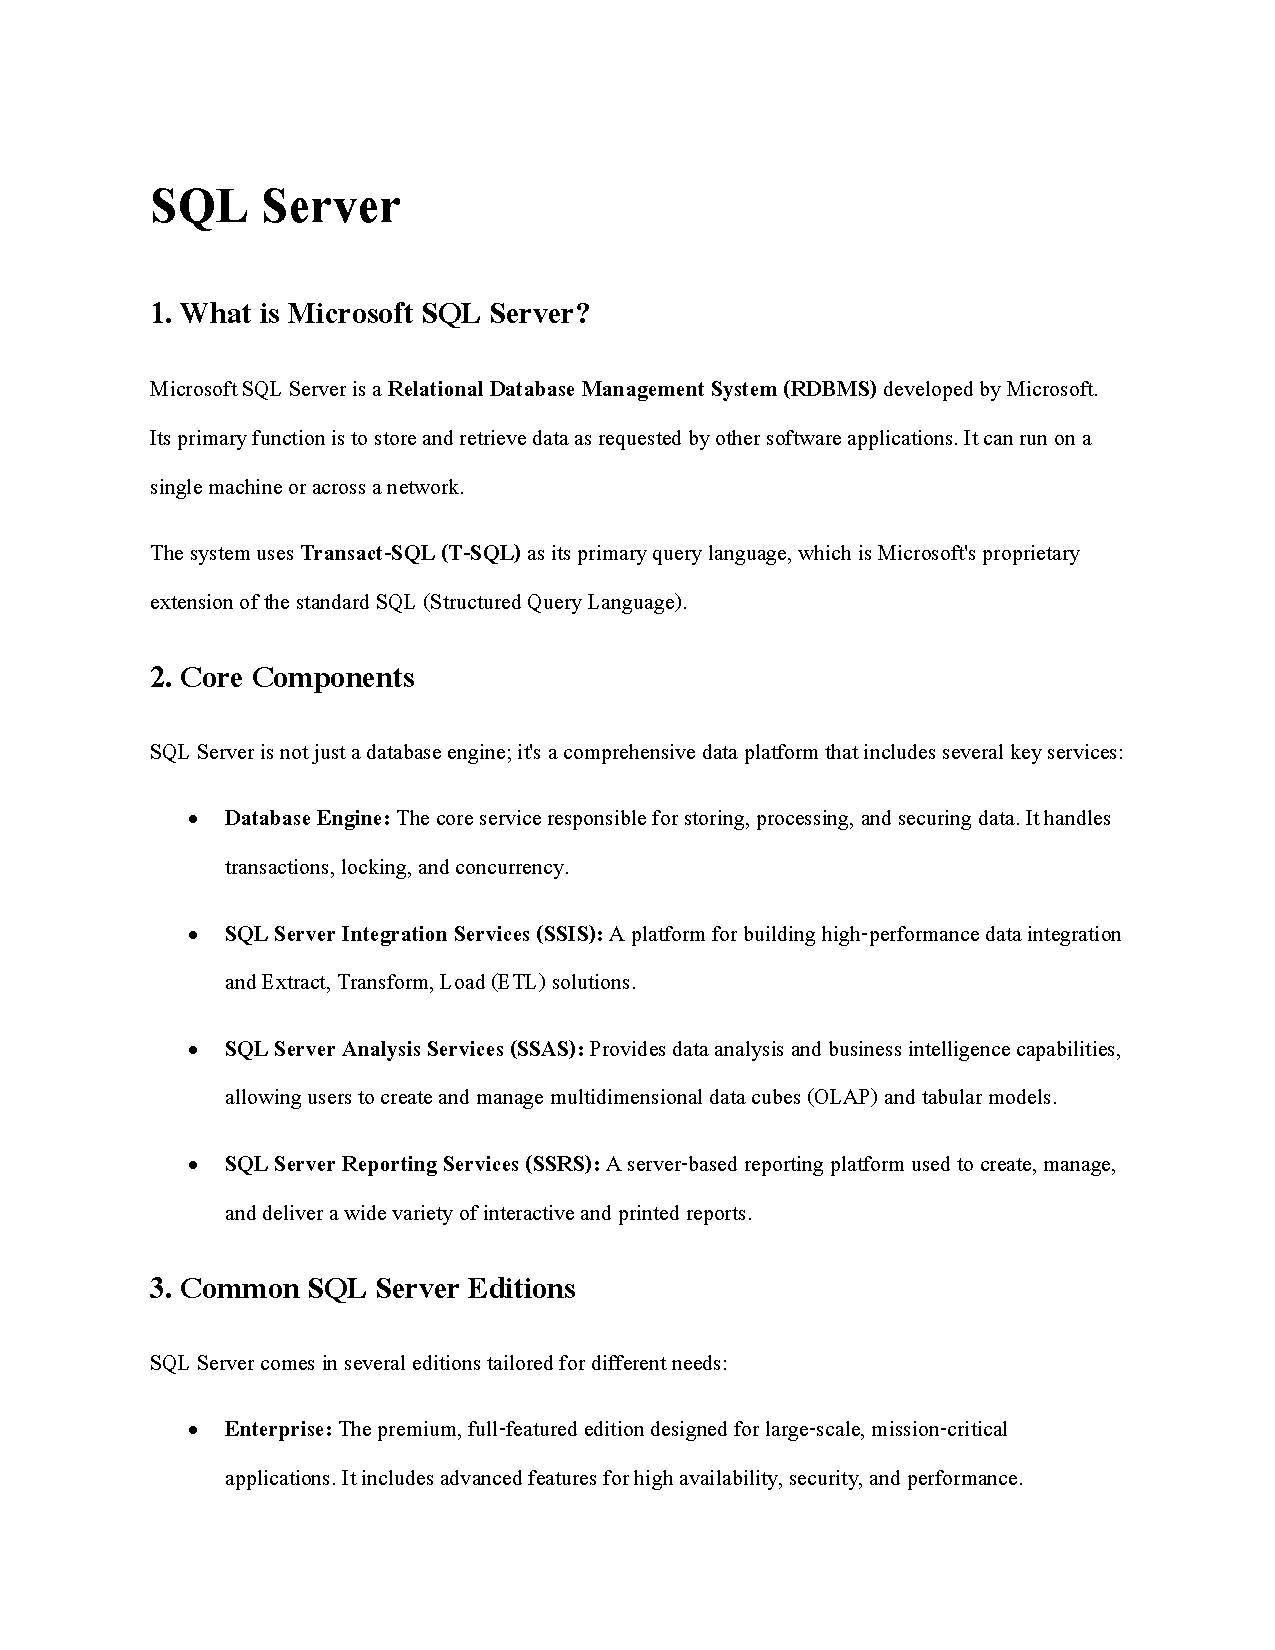
\includepdf[pages=-, scale=.8, pagecommand={\hypertarget{target:sqlserver}{},\label{page:sqlserver}}, nup=1x1, frame=false]{pdf/sqlserver}
